\documentclass[11pt, a4paper]{article}
\usepackage[utf8]{inputenc}
\usepackage{amsmath, amssymb}
\usepackage{graphicx}
\usepackage{booktabs}
\usepackage{tabularx}
\usepackage[margin=1in]{geometry}
\usepackage[dvipsnames]{xcolor}
\usepackage[hidelinks]{hyperref}
\usepackage{url}
\usepackage{float}
\usepackage[font=small, labelfont=bf, skip=6pt]{caption}
\usepackage{enumitem}
\usepackage{microtype}
\setlist{itemsep=2pt, topsep=4pt}

% ---------- colours used in diagrams (match the figures) ----------
\definecolor{navy}{HTML}{1F3A5F}
\definecolor{teal}{HTML}{2A7F78}
\definecolor{brick}{HTML}{C0392B}
\definecolor{greyblue}{HTML}{9AA5B1}

% ---------- figure helper: shows a placeholder box if the file is missing ----------
\newcommand{\placefig}[2][\linewidth]{%
  \IfFileExists{#2}{\includegraphics[width=#1]{#2}}{%
    \fbox{\parbox[c][5cm][c]{#1}{\centering\small\textit{Figure placeholder}\\[2pt]\texttt{\detokenize{#2}}}}}}



\title{Retail Markdown Pricing and Margin Impact Analysis:\\[2pt]
\large Measuring Incremental Lift, Price Elasticity and the Profitability of Discounts}
\author{Your Name {\setlength{\fboxsep}{0.2pt}\fcolorbox{white}{white}{\href{https://drive.google.com/your-link-here}{\small Project Link}}}}
\date{September 2026}

\begin{document}
\maketitle

\begin{abstract}
\noindent Retailers mark products down to move stock and lift sales, and a markdown almost always sells more units. Whether those extra units pay for the price given up is a different question. This project studies 43,400 personal-care and beauty products, each taken through four sequential rounds of markdowns, to measure how much a discount actually adds and what it does to revenue and contribution margin. Three results stand out. First, measuring lift against the original baseline badly misattributes the effect of later markdowns; lift has to be measured against the period immediately before each markdown. Second, demand is price-inelastic (median elasticity $-0.65$), and the response depends almost entirely on whether a category is in season: in-season products respond about 5.6 times more strongly to the same discount. Third, over the full markdown cycle revenue rose 10.7\% relative to a no-markdown counterfactual, while contribution margin fell 22.9\% under an assumed 40\% cost of goods. A simulation of alternative policies suggests stopping off-season markdowns and capping in-season discounts at around 10\%. The problem framing is adapted from Increff's markdown optimization case study; the data is synthetic.

\vspace{4pt}\noindent\textbf{Keywords:} markdown optimization, price elasticity, incremental lift, ANOVA, Tukey HSD, counterfactual analysis, contribution margin
\end{abstract}

% =====================================================================
\section{Introduction}
Markdowns are one of the most frequently used and least carefully measured levers in retail. A discount that moves more units looks successful on a sales report, yet it may simply transfer margin to customers who would have bought anyway. The decision has three parts: \emph{which} products to discount, \emph{how deep} to go, and \emph{when}. Getting it wrong in one direction leaves unsold stock; in the other, it gives away profit.

This project was inspired by Increff's case study on markdown optimization~\cite{increff}, which frames exactly this decision for a retailer. The aim was to practise the analysis that sits behind such a decision, end to end, on a public dataset. The work is organised around four questions:
\begin{enumerate}[label=\textbf{Q\arabic*.}]
  \item How much additional volume does a markdown actually generate, measured correctly?
  \item How sensitive is demand to price, and does that sensitivity vary by season, category or promotion channel?
  \item Do deeper discount tiers perform significantly differently from shallower ones?
  \item Taking cost into account, did the markdown programme create or destroy value, and what policy would have done better?
\end{enumerate}
The same logic applies well beyond apparel and beauty retail. Any business that runs coupons or promotions, including food delivery and quick commerce, faces the question of whether an incentive generates \emph{incremental} demand or subsidises demand that already existed.

% =====================================================================
\section{Data and Preprocessing}
\subsection{Dataset}
The analysis uses the \textit{Retail Markdown Optimization: Discounts \& Sales} dataset~\cite{kaggle}, a synthetic dataset modelled on a French personal-care and beauty retailer. Each row is a product, observed at a pre-markdown baseline and after each of four sequential markdowns. Table~\ref{tab:data} summarises the fields used.

\begin{table}[!htbp]
\centering\small
\caption{Dataset overview (after cleaning)}
\label{tab:data}
\begin{tabularx}{\textwidth}{lX}
\toprule
\textbf{Field} & \textbf{Description} \\
\midrule
Products & 43,400 unique products (43,750 raw rows) \\
Category & Skincare (19,530), Bodycare (13,020), Makeup (10,850) \\
Season, Brand, Channel & 4 seasons; 6 brands; promotion channel: in-store, online, social media \\
Prices & Original price 5--100 (mean 52.7); competitor price (mean 53.7) \\
Seasonality factor & Score from 0.5 to 2.0 (mean 1.33) \\
Baseline sales & Units sold before any markdown (mean 171.9, range 26--416) \\
Markdowns & Four rounds per product: 10--40\%, 20--50\%, 10--30\%, 30--50\% \\
Sales after markdown & Units sold after each of the four rounds \\
Not available & Product cost, calendar dates, stock figures consistent with sales \\
\bottomrule
\end{tabularx}
\end{table}

\subsection{Data quality}
Three issues were found and handled before any modelling:
\begin{itemize}
  \item \textbf{Duplicate records.} 350 rows were exact duplicates of other rows (same product ID and identical values in every column). They were removed, leaving 43,400 products.
  \item \textbf{A leaking column.} The dataset provides an ``Optimal Discount'' field. Its correlation with the mean of each product's four markdowns is 0.997, so it is derived from the inputs rather than being an independent benchmark. It was excluded; treating it as a target would amount to grading the markdowns against themselves.
  \item \textbf{No cost data.} Contribution margin requires cost of goods sold (COGS). COGS was therefore set as an assumption (40\% of original price) and tested at 30\% and 50\%.
\end{itemize}

\subsection{Reshaping to event level}
The four markdown and sales columns were unpivoted in SQL (DuckDB~\cite{duckdb}) into one row per product and markdown round, giving 173,600 markdown events. A \texttt{LAG} window function, partitioned by product and ordered by round, attached the previous period's sales to each event (Figure~\ref{fig:reshape}). The full SQL is linked under Code Availability.

\begin{figure}[!htbp]
\centering
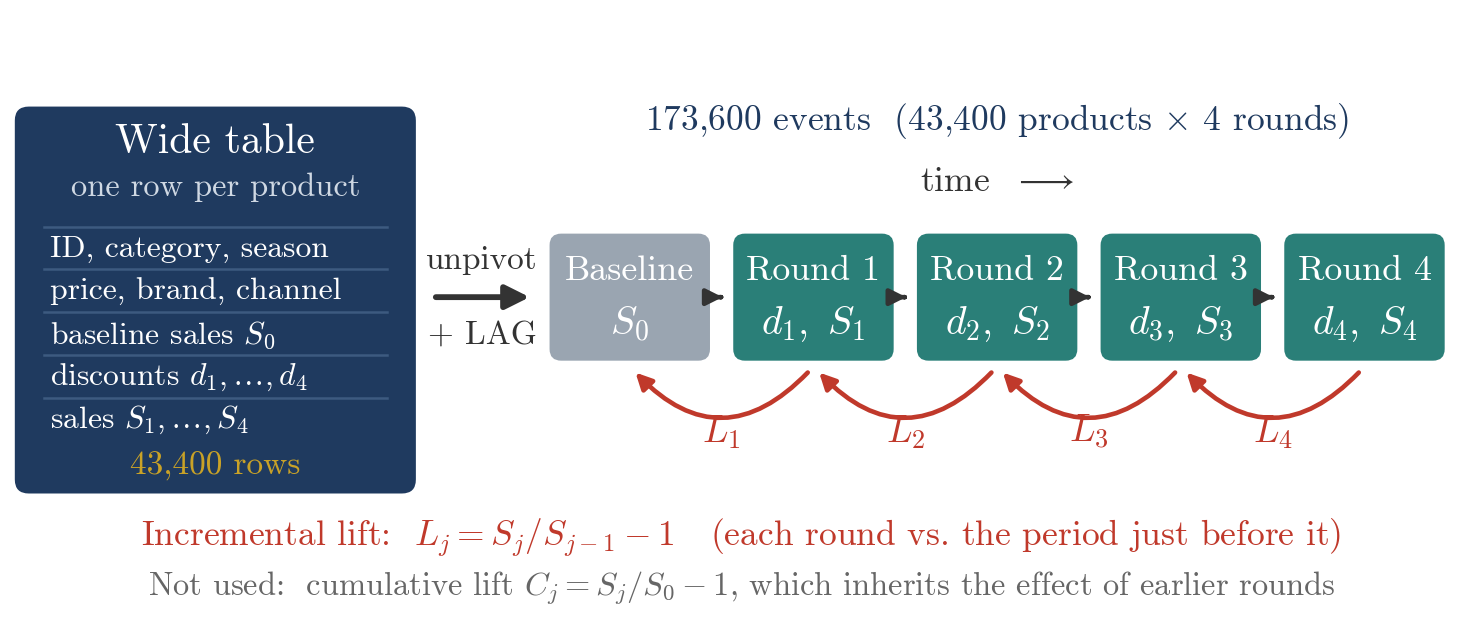
\includegraphics[width=0.9\linewidth]{fig00a_reshape.png}
\caption{Reshaping the wide product table into markdown events and defining incremental lift.}
\label{fig:reshape}
\end{figure}

Figure~\ref{fig:overview} shows the design of the four rounds and the distribution of lift. Rounds 1 and 3 are shallow, rounds 2 and 4 deep. Incremental lift has a mean of 17.9\% and a median of 16.7\%, with mild right skew (skewness 0.40).

\begin{figure}[!htbp]
\centering
\placefig[0.9\linewidth]{fig01_data_overview.pdf}
\caption{(a) Discount depth by round. (b) Distribution of incremental lift across all 173,600 markdown events.}
\label{fig:overview}
\end{figure}

% =====================================================================
\section{Methodology}
Figure~\ref{fig:pipeline} summarises the analysis. The key definitions are set out below.

\begin{figure}[!htbp]
\centering
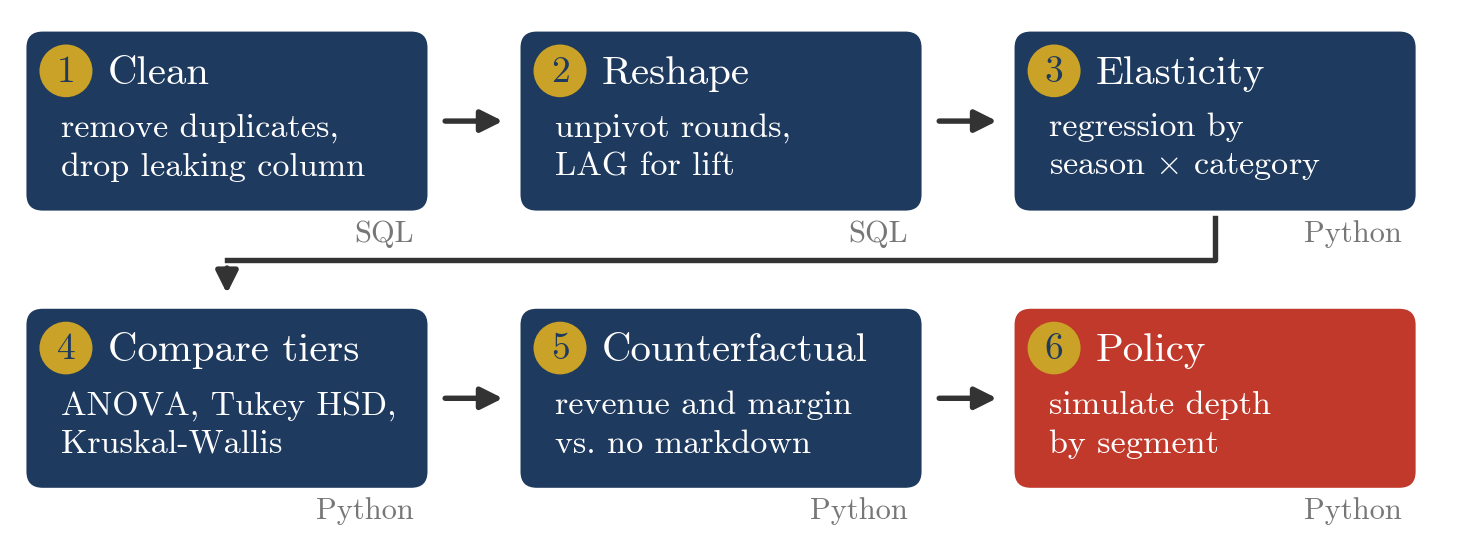
\includegraphics[width=0.78\linewidth]{fig00b_pipeline.png}
\caption{Analysis pipeline. Steps 1--2 run in SQL (DuckDB); steps 3--6 in Python (pandas, statsmodels, SciPy).}
\label{fig:pipeline}
\end{figure}

\subsection{Incremental lift and break-even}
For product $i$ in round $j \in \{1,\dots,4\}$ with discount $d_{ij}$ and unit sales $S_{ij}$ ($S_{i0}$ being the baseline), incremental and cumulative lift are
\begin{equation}
L_{ij} = \frac{S_{ij}}{S_{i,j-1}} - 1, \qquad C_{ij} = \frac{S_{ij}}{S_{i0}} - 1 .
\end{equation}
Because sales in this data carry forward from one round to the next, $C_{ij}$ mixes the effect of round $j$ with every earlier round. All analysis therefore uses $L_{ij}$. A markdown holds period revenue constant only if $(1-d)(1+L) \geq 1$, i.e.\ if lift reaches the break-even level
\begin{equation}
L^{\ast}(d) = \frac{d}{1-d},
\end{equation}
so a 30\% discount needs 43\% more units just to stand still on revenue.

\subsection{Price elasticity and the response model}
Event-level elasticity is $\varepsilon_{ij} = -L_{ij}/d_{ij}$, and medians are reported. Because lift turned out to be close to proportional to depth, the response is modelled without an intercept:
\begin{equation}
L_{ij} = d_{ij}\,\bigl(\beta_{s(i)} + \boldsymbol{\gamma}^{\top}\mathbf{x}_i\bigr) + \delta_j + u_{ij},
\end{equation}
where $\beta_{s(i)}$ is the response slope for product $i$'s season--category segment, $\mathbf{x}_i$ contains promotion channel, brand and the price gap to competitors, and $\delta_j$ are round effects. Four specifications were compared (M1: depth only; M2: depth $\times$ seasonality factor; M3: depth $\times$ season $\times$ category; M4: M3 plus the seasonality factor). Each product contributes four correlated events, so standard errors are clustered by product~\cite{cameron}.

\subsection{Comparing discount tiers}
Events were grouped into four depth tiers (10--20\%, 20--30\%, 30--40\%, 40--50\%). A one-way ANOVA assumes independent observations, which the four rounds of the same product are not. To respect this, \textbf{one round was drawn at random from each product}, giving 43,400 independent observations. Differences were tested with a one-way ANOVA (effect size $\eta^2$), checked with the non-parametric Kruskal--Wallis test~\cite{kruskal}, and followed by Tukey's HSD~\cite{tukey} for all six pairwise comparisons at a family-wise error rate of 5\%.

\subsection{Counterfactual revenue and margin}
Actual outcomes over the four rounds were compared with a counterfactual in which every product stays at full price and baseline volume. With original price $P_i$ and COGS fraction $c$:
\begin{align}
R^{\text{act}}_i &= \textstyle\sum_{j=1}^{4} P_i (1-d_{ij}) S_{ij}, & R^{\text{cf}}_i &= 4 P_i S_{i0}, \\
M^{\text{act}}_i &= \textstyle\sum_{j=1}^{4} P_i (1-d_{ij}-c)\, S_{ij}, & M^{\text{cf}}_i &= 4 P_i (1-c)\, S_{i0}.
\end{align}

\subsection{Policy simulation}
For each segment $s$, a uniform depth $d \in \{10\%, 15\%, \dots, 50\%\}$ was held for four rounds, with sales compounding as $S_j = S_0 (1 + \hat\beta_s d)^j$. Revenue and margin were compared with the counterfactual, and the revenue-maximising and margin-maximising depths recorded. Depths below 10\% were not simulated because the data contains none.

% =====================================================================
\section{Results}
\subsection{Cumulative measurement misattributes lift}
Table~\ref{tab:rounds} and Figure~\ref{fig:attr} contrast the two ways of measuring lift. Under the cumulative view, round 3 (mean depth 20\%) appears to outperform round 2 (35\%), 58.3\% against 40.0\%. That result is an artefact: round 3 inherits the growth of the two rounds before it. Measured incrementally, round 3 added 11.9\% and round 2 added 20.9\%, the ordering one would expect from their depths. A team working from the cumulative numbers would favour exactly the wrong markdowns.

\begin{table}[!htbp]
\centering\small
\caption{Markdown rounds: depth, incremental and cumulative lift, and break-even lift (computed in SQL)}
\label{tab:rounds}
\setlength{\tabcolsep}{5pt}
\begin{tabular}{lcccccc}
\toprule
 & \textbf{Depth} & \textbf{Mean} & \multicolumn{2}{c}{\textbf{Incremental lift}} & \textbf{Cumulative} & \textbf{Break-even} \\
\cmidrule(lr){4-5}
\textbf{Round} & \textbf{range} & \textbf{depth} & \textbf{mean} & \textbf{median} & \textbf{lift} & \textbf{lift} \\
\midrule
1 & 10--40\% & 25.1\% & 15.0\% & 14.0\% & 15.0\%  & 35.3\% \\
2 & 20--50\% & 35.0\% & 20.9\% & 21.2\% & 40.0\%  & 56.7\% \\
3 & 10--30\% & 20.0\% & 11.9\% & 11.7\% & 58.3\%  & 25.6\% \\
4 & 30--50\% & 40.0\% & 23.9\% & 25.5\% & 100.8\% & 68.3\% \\
\bottomrule
\end{tabular}
\end{table}

\begin{figure}[!htbp]
\centering
\placefig[0.9\linewidth]{fig02_attribution.pdf}
\caption{Cumulative versus incremental lift by round.}
\label{fig:attr}
\end{figure}

\subsection{Demand response depends on season fit, not on the seasonality score}
Lift rises almost linearly with depth, so the useful quantity is the slope: how many points of lift each point of discount buys. Depth alone explains 21\% of the variation in lift (Table~\ref{tab:models}). Letting the slope depend on the dataset's seasonality factor raises this to 49\%, and the factor's coefficient is large and highly significant (0.497). Letting the slope depend on season and category instead raises it to 79\%.

\begin{table}[!htbp]
\centering\small
\caption{Response models for incremental lift (no intercept; standard errors clustered by product)}
\label{tab:models}
\begin{tabular}{llcc}
\toprule
\textbf{Model} & \textbf{Depth interacted with} & $\boldsymbol{R^2}$ & \textbf{Seas.\ factor coef.} \\
\midrule
M1 & nothing & 0.212 & -- \\
M2 & seasonality factor + controls & 0.486 & 0.497 ($p<0.001$) \\
M3 & season $\times$ category + controls & 0.791 & -- \\
M4 & M3 + seasonality factor & 0.791 & 0.0002 ($p=0.95$) \\
\bottomrule
\end{tabular}
\end{table}

M4 settles what drives the response. Once season and category are in the model, the seasonality factor has no effect at all ($p = 0.95$). It looked important in M2 only because it is high for most in-season combinations, so it was acting as a proxy for the real driver. The estimated slopes fall into two clear groups (Figure~\ref{fig:models}): eight in-season segments with a slope of about 0.85, and four off-season segments (Makeup and Skincare in the rainy season; Bodycare and Skincare in Spring) with a slope of about 0.15. The same discount therefore buys roughly 5.6 times more lift when a category is in season. None of the control variables matter: promotion channel ($p = 0.74$ and $0.46$), the price gap to competitors ($p = 0.78$) and round ($p > 0.77$) are all insignificant.

\begin{figure}[!htbp]
\centering
\placefig[0.9\linewidth]{fig05_models.pdf}
\caption{(a) Explained variance of models M1--M4. (b) Estimated response slope $\hat\beta_s$ for each season--category segment.}
\label{fig:models}
\end{figure}

In elasticity terms, demand is inelastic everywhere: the median across all events is $-0.65$, in-season segments sit at $-0.85$ and off-season segments at $-0.15$ (Figure~\ref{fig:elast}). The marginal medians in panel (b) are averages over this pattern. Skincare's lower figure ($-0.50$), for instance, only reflects that it is off season in two of the four seasons; in season it responds like any other category.

\begin{figure}[!htbp]
\centering
\placefig[0.9\linewidth]{fig04_elasticity.pdf}
\caption{(a) Median price elasticity by season and category. (b) Marginal medians by season, by category and overall.}
\label{fig:elast}
\end{figure}

Figure~\ref{fig:regime} places both groups against the break-even curve. Neither comes close at any depth, which is why only 0.6\% of all markdown events (0.97\% in season, none off season) recovered their own discount within the period.

\begin{figure}[!htbp]
\centering
\placefig[0.9\linewidth]{fig03_lift_by_regime.pdf}
\caption{Incremental lift by discount depth for in-season and off-season products (95\% CIs), against the break-even lift $d/(1-d)$.}
\label{fig:regime}
\end{figure}

\subsection{Discount tiers differ significantly, and deeper tiers lose more revenue}
The four tiers differ significantly in lift: $F = 3{,}434$, $p < 0.001$, $\eta^2 = 0.19$. The Kruskal--Wallis test agrees ($H = 7{,}678$, $p < 0.001$). Tukey's HSD finds every one of the six pairs significantly different, both for unit lift and for period revenue (Table~\ref{tab:tukey}, Figure~\ref{fig:tiers}). Each 10-point step in depth adds about 6 points of lift, and each step also loses revenue for the period, from $-7.2\%$ in the shallowest tier to $-30.0\%$ in the deepest (Table~\ref{tab:tiers}). There is no sweet spot where a deeper cut starts to pay.

\begin{table}[!htbp]
\centering\small
\caption{Outcomes by discount tier (one randomly selected round per product)}
\label{tab:tiers}
\begin{tabular}{lcccc}
\toprule
\textbf{Tier} & \textbf{$n$} & \textbf{Unit lift} & \textbf{95\% CI} & \textbf{Period revenue change} \\
\midrule
10--20\% & 8,653  & 8.9\%  & $\pm$0.1 pp & $-7.2\%$ \\
20--30\% & 12,402 & 14.7\% & $\pm$0.2 pp & $-13.5\%$ \\
30--40\% & 12,749 & 20.6\% & $\pm$0.2 pp & $-21.1\%$ \\
40--50\% & 9,596  & 26.6\% & $\pm$0.4 pp & $-30.0\%$ \\
\bottomrule
\end{tabular}
\end{table}

\begin{table}[!htbp]
\centering\small
\caption{Tukey HSD pairwise comparisons of unit lift (percentage points)}
\label{tab:tukey}
\begin{tabular}{lccc}
\toprule
\textbf{Comparison} & \textbf{Mean difference} & \textbf{95\% family-wise CI} & \textbf{Adjusted $p$} \\
\midrule
20--30\% vs 10--20\% & 5.85  & [5.40, 6.31]   & $<0.001$ \\
30--40\% vs 10--20\% & 11.71 & [11.26, 12.16] & $<0.001$ \\
40--50\% vs 10--20\% & 17.71 & [17.22, 18.19] & $<0.001$ \\
30--40\% vs 20--30\% & 5.86  & [5.45, 6.27]   & $<0.001$ \\
40--50\% vs 20--30\% & 11.85 & [11.41, 12.29] & $<0.001$ \\
40--50\% vs 30--40\% & 6.00  & [5.56, 6.43]   & $<0.001$ \\
\bottomrule
\end{tabular}
\end{table}

\begin{figure}[!htbp]
\centering
\begin{minipage}{0.49\textwidth}\centering\placefig{fig06_tiers.pdf}\end{minipage}\hfill
\begin{minipage}{0.49\textwidth}\centering\placefig{fig07_tukey.pdf}\end{minipage}
\caption{Left: unit lift (bars, 95\% CI) and period revenue change (line) by tier. Right: Tukey HSD intervals; none crosses zero.}
\label{fig:tiers}
\end{figure}

\subsection{Revenue rose, contribution margin fell}
Against the no-markdown counterfactual, the extra volume was worth 61.1 index points of revenue at full price and the discounts gave back 50.4, leaving revenue 10.7\% higher (Figure~\ref{fig:waterfall}). Margin behaves differently: each extra unit carries its own cost, while the discount comes directly out of profit. Contribution margin ended 22.9\% below the counterfactual, and 97.9\% of products were worse off.

\begin{figure}[!htbp]
\centering
\placefig[0.9\linewidth]{fig09_waterfall.pdf}
\caption{Decomposition of revenue and contribution margin over the four rounds (no markdown = 100).}
\label{fig:waterfall}
\end{figure}

The conclusion does not depend on the cost assumption (Table~\ref{tab:cf}): margin falls at every COGS level tested. Splitting by season fit sharpens it further. In-season products gained revenue but still lost margin; off-season products lost on both.

\begin{table}[!htbp]
\centering\small
\caption{Change vs.\ the no-markdown counterfactual: sensitivity to COGS, and split by season fit (COGS = 40\%; computed in SQL)}
\label{tab:cf}
\begin{tabular}{lccc}
\toprule
\textbf{Scenario} & \textbf{Revenue} & \textbf{Contribution margin} & \textbf{Products losing margin} \\
\midrule
COGS 30\% & +10.7\% & $-10.9\%$ & 76.6\% \\
COGS 40\% & +10.7\% & $-22.9\%$ & 97.9\% \\
COGS 50\% & +10.7\% & $-39.7\%$ & 100.0\% \\
\midrule
In-season products  & +21.6\% & $-15.7\%$ & -- \\
Off-season products & $-22.5\%$ & $-44.9\%$ & -- \\
\bottomrule
\end{tabular}
\end{table}

\subsection{Policy simulation: revenue and margin point in opposite directions}
Figure~\ref{fig:policy} shows the simulated outcome of holding one depth for all four rounds. For in-season segments, revenue keeps rising up to 45\% off, reaching about 32\% above the counterfactual. A team that sets discounts to maximise revenue or GMV would choose that depth, and would lose about 40\% of contribution margin in the process. Margin is highest at 10\% (about +2.7\%) and turns negative a little past 20\%. For off-season segments, every depth loses both revenue and margin; the least damaging option, 10\%, still costs 13.5\% of margin.

\begin{figure}[!htbp]
\centering
\placefig[0.9\linewidth]{fig10_policy.pdf}
\caption{Simulated revenue and contribution margin against a uniform discount depth (COGS = 40\%).}
\label{fig:policy}
\end{figure}

% =====================================================================
\section{Discussion and Recommendations}
The evidence points to a small number of concrete changes (Table~\ref{tab:recs}). The broader lesson is about measurement: this markdown programme looked successful on units and revenue, and was loss-making on the metric that matters. Discount decisions should be judged on incremental units and contribution margin, with revenue as a supporting number.

\begin{table}[!htbp]
\centering\small
\caption{Recommendations}
\label{tab:recs}
\begin{tabularx}{\textwidth}{>{\raggedright\arraybackslash}p{5.2cm}X}
\toprule
\textbf{Recommendation} & \textbf{Evidence} \\
\midrule
Stop marking down off-season products & Revenue $-22.5\%$ and margin $-44.9\%$ vs.\ no markdown; no depth breaks even \\
Cap in-season markdowns near 10\% (current average: 30\%) & 10\% was the margin-maximising depth in all eight in-season segments \\
Do not set depth by revenue & Revenue peaks at 45\% off, where margin is about 40\% below the counterfactual \\
Stop paying a premium for any one promotion channel & No difference between in-store, online and social media \\
Report markdowns on incremental lift and margin & Cumulative lift mis-ranked the markdown rounds \\
\bottomrule
\end{tabularx}
\end{table}

One qualification matters. Markdowns also exist to clear stock that would otherwise be written off. This analysis gives unsold stock no cost, which favours shallow discounts. For aged or end-of-season inventory, a deeper markdown can still be the right decision, and judging that would require holding costs and salvage values.

% =====================================================================
\section{Limitations and Future Work}
\begin{itemize}
  \item \textbf{Synthetic data.} The patterns reflect how the data was generated; the sharp two-group structure in Figure~\ref{fig:models} is an example. The method, not the specific numbers, is what transfers to real data.
  \item \textbf{No undiscounted control.} Every product was discounted in every round, so a general trend cannot be fully separated from the discount effect. Results should be read as strong associations, not proven causal effects.
  \item \textbf{Assumed cost.} COGS was not observed, hence the sensitivity analysis.
  \item \textbf{Inventory not modelled.} The stock column did not reconcile with sales and was not used.
  \item \textbf{Limited depth range.} The data contains no discounts below 10\%, so shallower policies cannot be evaluated.
\end{itemize}
With real transaction data, the natural next steps are a randomised holdout of products kept at full price to measure lift causally; adding cost, stock age and sell-through so that margin can be traded against the cost of unsold inventory; and estimating elasticity at the product level to set markdowns per SKU.

% =====================================================================
\section{Conclusion}
This project measured what a four-round markdown programme actually achieved for 43,400 products. Correctly measured, discounts added volume, but demand was inelastic (median elasticity $-0.65$) and the response depended mainly on whether a category was in season. All four discount tiers differed significantly, and each deeper tier lost more revenue than the last. Over the full cycle, revenue rose 10.7\% while contribution margin fell 22.9\%. The recommended policy is to stop off-season markdowns and to cap in-season discounts near 10\%, and to judge every markdown on incremental units and margin rather than on sales or revenue.

\section*{Tools and Environment}
\begin{itemize}
  \item \textbf{SQL:} DuckDB, for auditing, de-duplication, unpivoting, CTEs, window functions and \texttt{ROLLUP} aggregation (script linked below).
  \item \textbf{Python:} pandas, NumPy, statsmodels~\cite{statsmodels} (OLS with cluster-robust errors, Tukey HSD), SciPy (ANOVA, Kruskal--Wallis), matplotlib.
  \item \textbf{Validation:} random one-event-per-product sampling for ANOVA, non-parametric cross-check, COGS sensitivity analysis.
\end{itemize}

\section*{Code Availability}
The complete SQL pipeline (DuckDB) is available here: \href{https://drive.google.com/your-sql-file-link}{\texttt{markdown\_pricing\_analysis.sql}}. It runs end to end from the raw CSV and covers the data audit and de-duplication, the unpivot of the four markdown rounds, incremental lift with \texttt{LAG}, the round-level comparison in Table~\ref{tab:rounds}, and the season-fit counterfactual in Table~\ref{tab:cf}. The expected output is noted under each query.

\begin{thebibliography}{9}
\bibitem{increff} Increff. \textit{Markdown Optimization Case Study}. [Add the link to the case study you used.]
\bibitem{kaggle} A.~Tamboli. \textit{Retail Markdown Optimization: Discounts \& Sales} [Dataset]. Kaggle. \url{https://www.kaggle.com/datasets/arbaaztamboli/retail-markdown-optimization-discounts-and-sales}
\bibitem{tukey} J.~W.~Tukey (1949). Comparing individual means in the analysis of variance. \textit{Biometrics}, 5(2), 99--114.
\bibitem{kruskal} W.~H.~Kruskal and W.~A.~Wallis (1952). Use of ranks in one-criterion variance analysis. \textit{Journal of the American Statistical Association}, 47(260), 583--621.
\bibitem{cameron} A.~C.~Cameron and D.~L.~Miller (2015). A practitioner's guide to cluster-robust inference. \textit{Journal of Human Resources}, 50(2), 317--372.
\bibitem{duckdb} M.~Raasveldt and H.~M\"uhleisen (2019). DuckDB: an embeddable analytical database. \textit{Proceedings of the 2019 International Conference on Management of Data (SIGMOD)}, 1981--1984.
\bibitem{statsmodels} S.~Seabold and J.~Perktold (2010). statsmodels: Econometric and statistical modeling with Python. \textit{Proceedings of the 9th Python in Science Conference}.
\end{thebibliography}

\end{document}
